\section{Clustering measurements}
\label{sec:clustering}
% =====================================================================

\subsection{Subvolumes and estimator}

Each $2\,h^{-1}$Gpc box is divided into $4^3=64$ non-overlapping cubic subvolumes of $500\Mpch$ (about $62\,500$ galaxies each). Each subvolume is treated as an independent survey with open boundaries: correlation functions are measured with the Landy--Szalay estimator \cite{LandySzalay1993},
\begin{equation}
\xi(s,\mu) = \frac{D_1D_2 - D_1R - RD_2 + RR}{RR},
\end{equation}
using a uniform catalogue of $5\times$ the number of galaxies to describe the geometry (the same for all subvolumes, so that $RR$ is computed once). Here $D_1D_2$ counts the pairs of points of the two samples at separation $s$, $D_1R$ and $RD_2$ the pairs between each sample and the random catalogue, and $RR$ the pairs of random points: $RR$ gives the number of pairs expected in this geometry if there were no clustering, and the combination corrects for the edges of the subvolume. Pair counts are computed with \texttt{pycorr}/\texttt{Corrfunc} \cite{Sinha2020} in 30 bins of $5\Mpch$ in $s\in[0,150]\Mpch$ and 120 bins in $\mu\in[-1,1]$, with $\mu$ defined with respect to the fixed line of sight, and projected on the Legendre multipoles $\ell=0,2,4$ (only $\ell=0,2$ are used in the forecasts).

\subsection{Statistics}

For each method $m\in\{$ASTRA, DS$\}$, population $p\in\{$random, galaxy$\}$ and quartile Q$_i$ we measure two statistics, together with the galaxy two-point correlation function $\xi^{\rm GG}_\ell(s)$ (2PCF), the excess probability of finding two galaxies at separation $s$: 33 statistics per catalogue.
\begin{itemize}
\item The \emph{quartile--galaxy cross-correlation} $\xi^{\rm QG}_{i,\ell}(s)$, between the points of Q$_i$ and all the galaxies: the average density of galaxies at distance $s$ from the points of the quartile, i.e.\ the mean galaxy profile around these environments (negative at small $s$ around voids, positive around clusters).
\item The \emph{quartile auto-correlation} $\xi^{\rm QQ}_{i,\ell}(s)$, between the points of Q$_i$ themselves: how the environments of one type are distributed in space relative to each other.
\end{itemize}
The first describes the shape of the structures, the second their large-scale distribution; both depend on cosmology. For random quartiles, they are the density-split cross- and auto-correlation functions of \cite{Paillas2023}. For galaxy quartiles, which split the galaxies into four sets of exactly equal size, the average of the four quartile--galaxy cross-correlations is the 2PCF, up to a negligible difference in the normalisation of the pair counts: every galaxy pair counted in the 2PCF is counted once in one of the four cross-correlations, the four quartiles share the same random catalogue, and with equal sizes the normalised pair counts, and hence the Landy--Szalay estimator, which is linear in them, simply average. The quartiles therefore decompose the 2PCF by environment, and it is this decomposition that adds information.

\subsection{Results on the fiducial cosmology}

Figure~\ref{fig:multipoles} compares the extreme quartiles of the two methods, and Figures~\ref{fig:mp_astra} and~\ref{fig:mp_ds} show all four quartiles of each method in the layout of the density-split analyses \cite{Paillas2023}; the galaxy quartiles are shown in Figure~\ref{fig:multipoles_gal}.

The two methods produce qualitatively identical signals, which have a simple physical reading. The Q1--galaxy cross-correlation is negative at small separations: it is the galaxy profile around underdense regions, which contain fewer galaxies than average out to $\sim50\Mpch$. The Q4--galaxy cross-correlation is positive and above the galaxy 2PCF: around overdense regions the galaxy density is higher than around an average galaxy. The auto-correlations of the extreme quartiles are much larger than the 2PCF: extreme environments, both dense and empty, are strongly clustered among themselves, because they are not placed at random but trace the large-scale modes of the density field, which they sample with a large (positive or negative) bias. This amplification is why environment statistics are sensitive to the amplitude and shape of the large-scale fluctuations. The quadrupoles have opposite signs for Q1 and Q4: around underdense regions peculiar velocities point outwards and stretch the void profile along the line of sight (positive quadrupole), while around overdense regions infall compresses it (negative quadrupole); they measure the growth rate of structure. The intermediate quartiles Q2 and Q3 have weak cross-correlations of opposite signs, close to the mean field, and auto-correlations 5--6 times below those of the extreme quartiles: most of the signal comes from the extremes.

The ASTRA signals are systematically weaker, by a factor $\sim1.6$ at the peak of the Q1 and Q4 cross-correlations ($s^2\xi_0\simeq-90$ and $+90\,h^{-2}{\rm Mpc}^2$, against $-145$ and $+145$ for density split). The reason is that ASTRA estimates the environment of each point from only $\sim15$ Delaunay neighbours, a noisy estimate: a point in a genuinely average region can, by chance, have mostly galaxy neighbours and be ranked in Q4. Each ASTRA quartile therefore contains a fraction of points that belong to other environments, which dilutes the contrast between quartiles (this is the mixing of Figure~\ref{fig:env}); density split averages over $\sim10\Mpch$, which reduces this noise. For density split the Q1 and Q4 auto-correlations are nearly equal, whereas for ASTRA the Q1 auto-correlation peaks 40\% above the Q4 one: ASTRA's underdense quartile is relatively more clustered with itself, a first sign that its auto-correlations carry distinct information. A weaker signal does not mean less information: what matters is the response of the signal to the parameters relative to its noise, which the forecasts address.

\begin{figure*}[!tp]
\centering
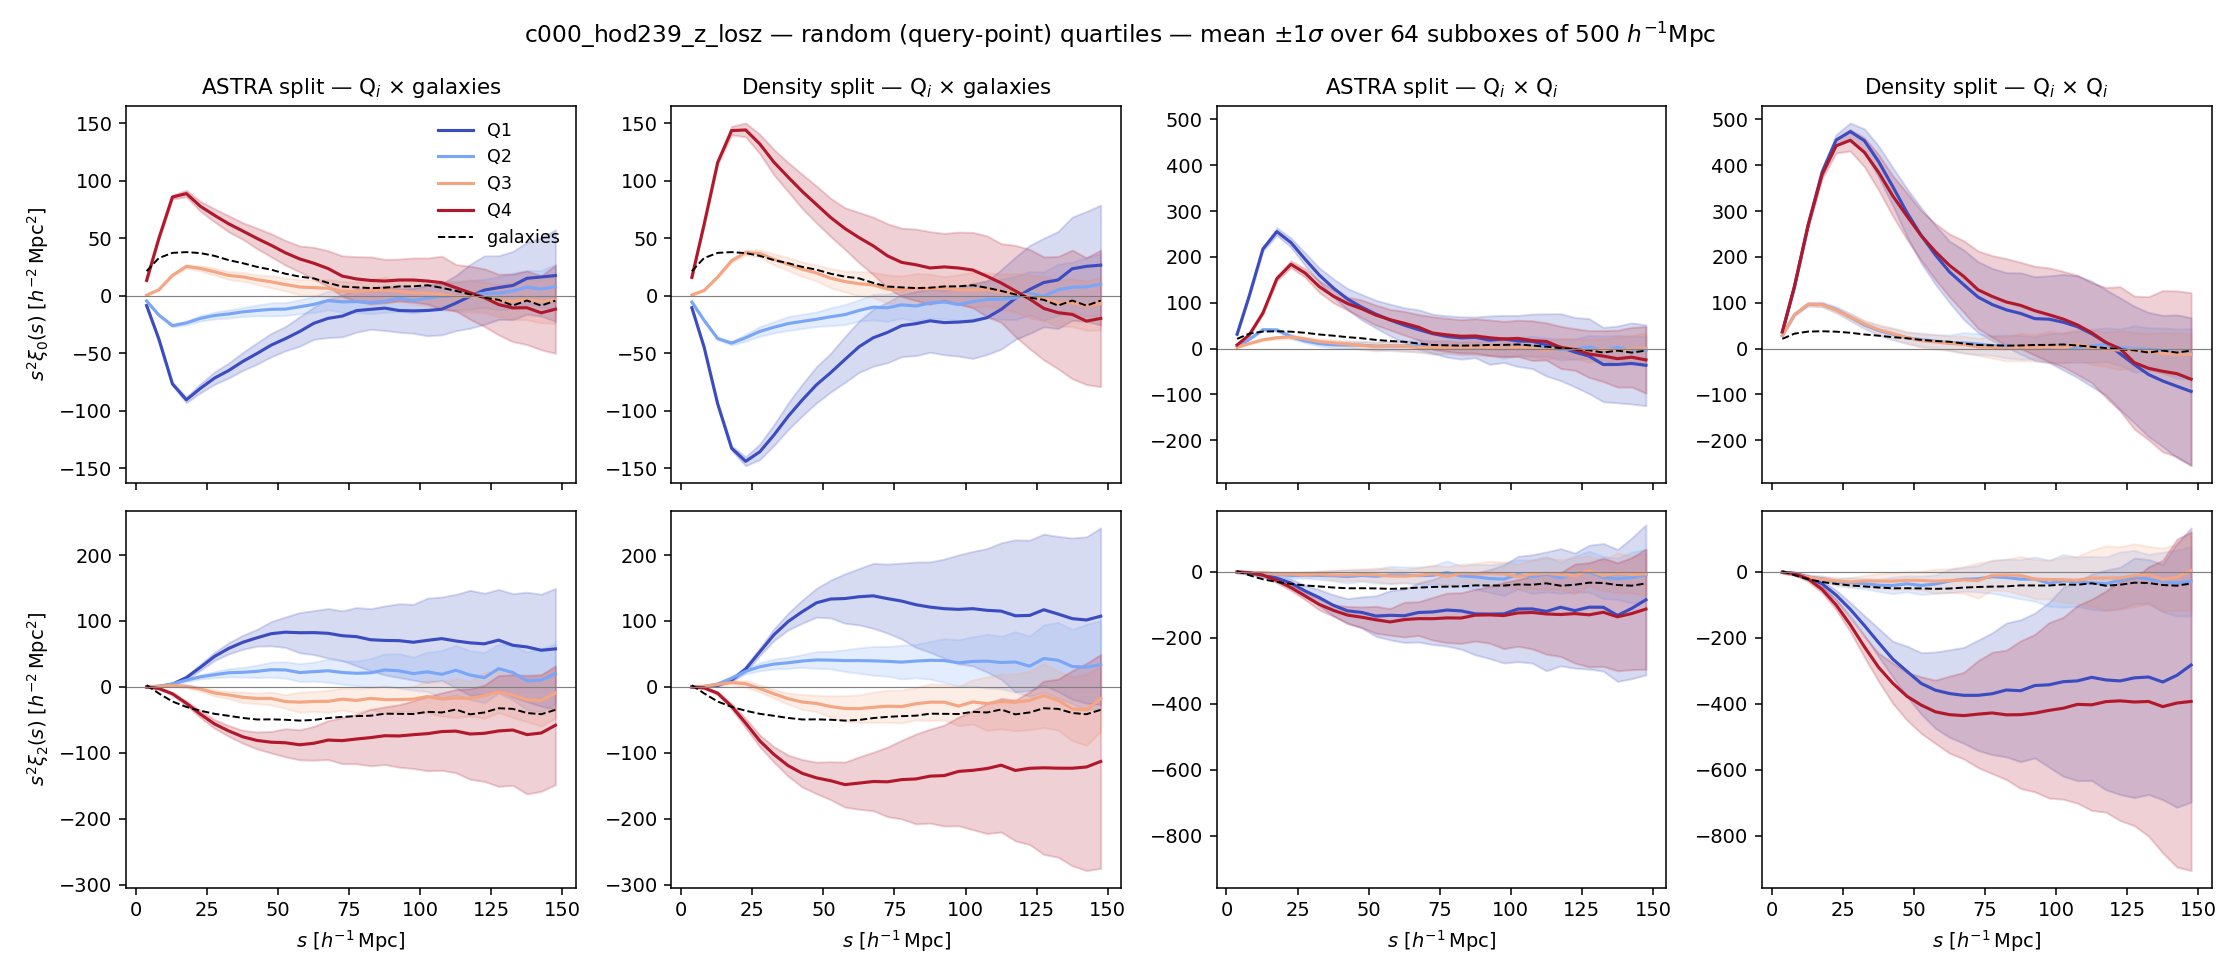
\includegraphics[width=\textwidth]{v2_multipoles_rand.png}
\caption{Monopole (top) and quadrupole (bottom) of the random-quartile statistics on the fiducial catalogue, for ASTRA split and density split: quartile--galaxy cross-correlations (left two columns) and quartile auto-correlations (right two columns), from Q1 (blue) to Q4 (red); dashed: galaxy 2PCF. Mean and $1\sigma$ scatter over the 64 subvolumes of $(500\Mpch)^3$; panels of the same statistic share the same scale.}
\label{fig:multipoles}
\end{figure*}

\begin{figure}[!htbp]
\centering
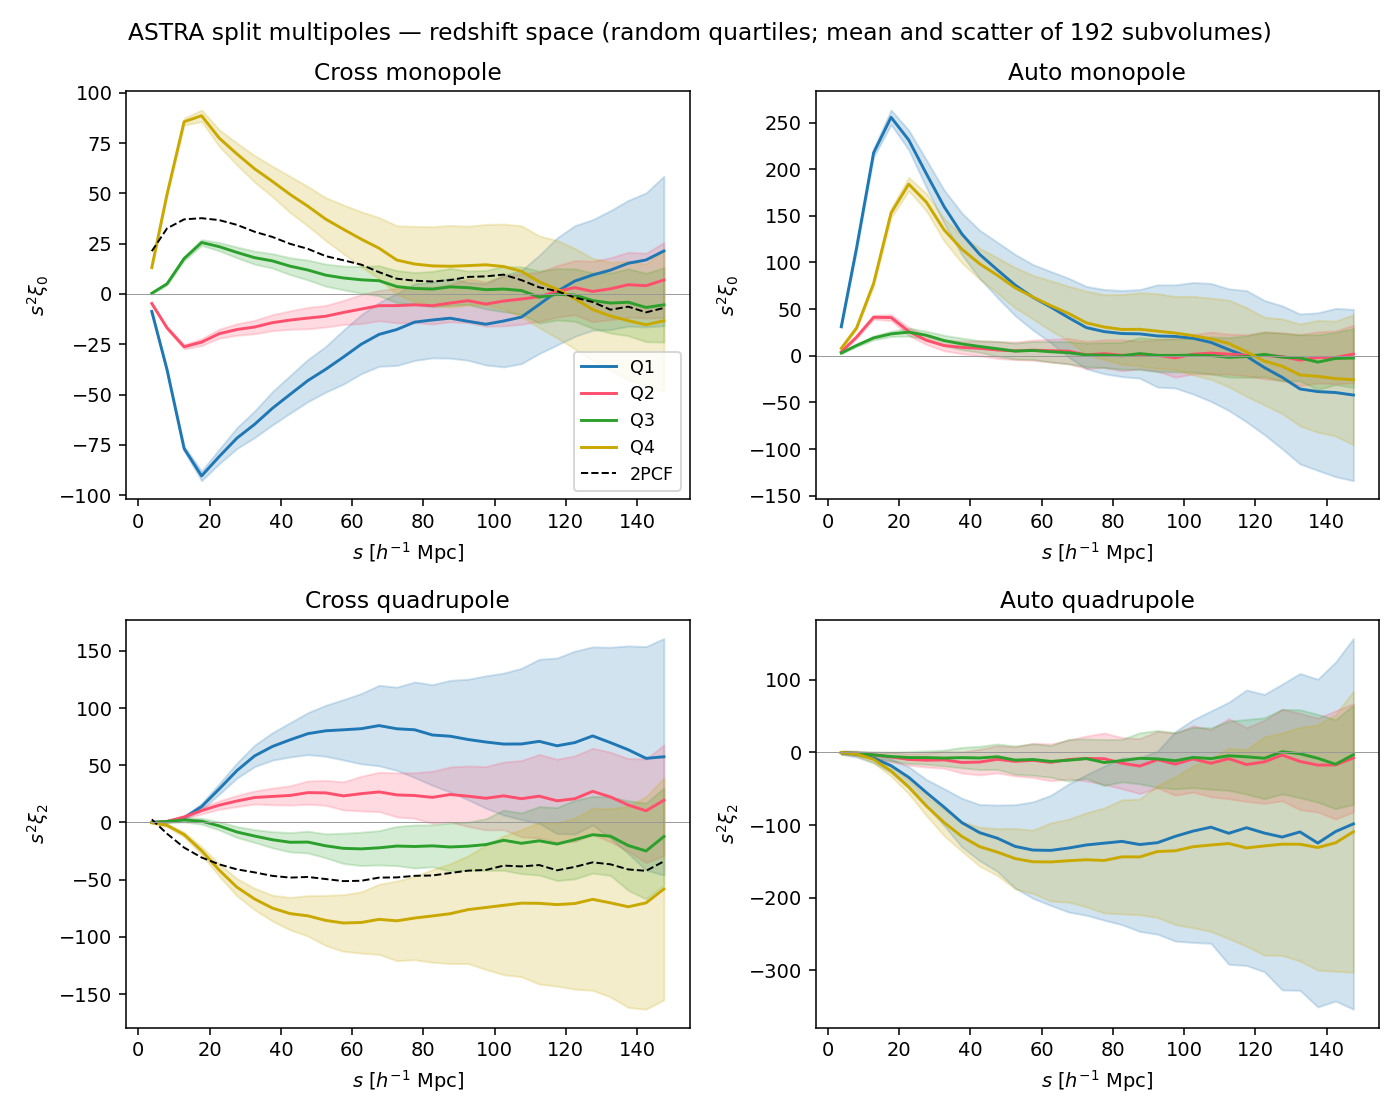
\includegraphics[width=\linewidth]{v1style_multipoles_astra.png}
\caption{ASTRA split: monopole and quadrupole of the quartile--galaxy cross-correlations (left) and quartile auto-correlations (right) for the four random quartiles; dashed: galaxy 2PCF. Mean and scatter of 192 subvolumes of the fiducial catalogue.}
\label{fig:mp_astra}
\end{figure}

\begin{figure}[!htbp]
\centering
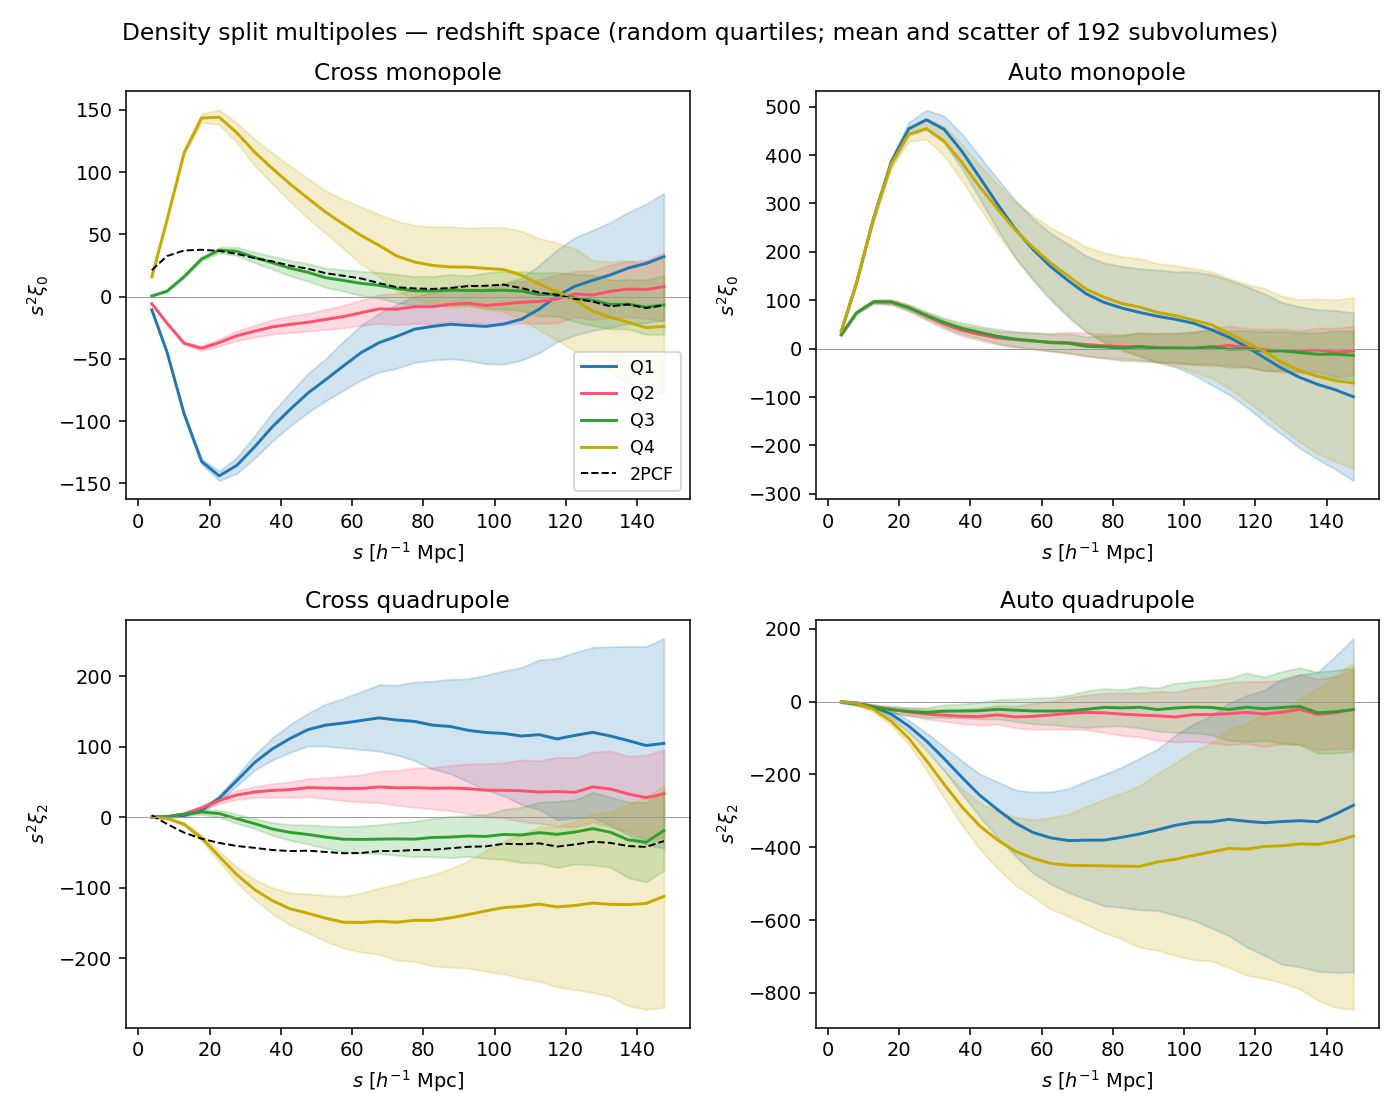
\includegraphics[width=\linewidth]{v1style_multipoles_ds.png}
\caption{Same as Figure~\ref{fig:mp_astra} for density split.}
\label{fig:mp_ds}
\end{figure}

\begin{figure*}[!tp]
\centering
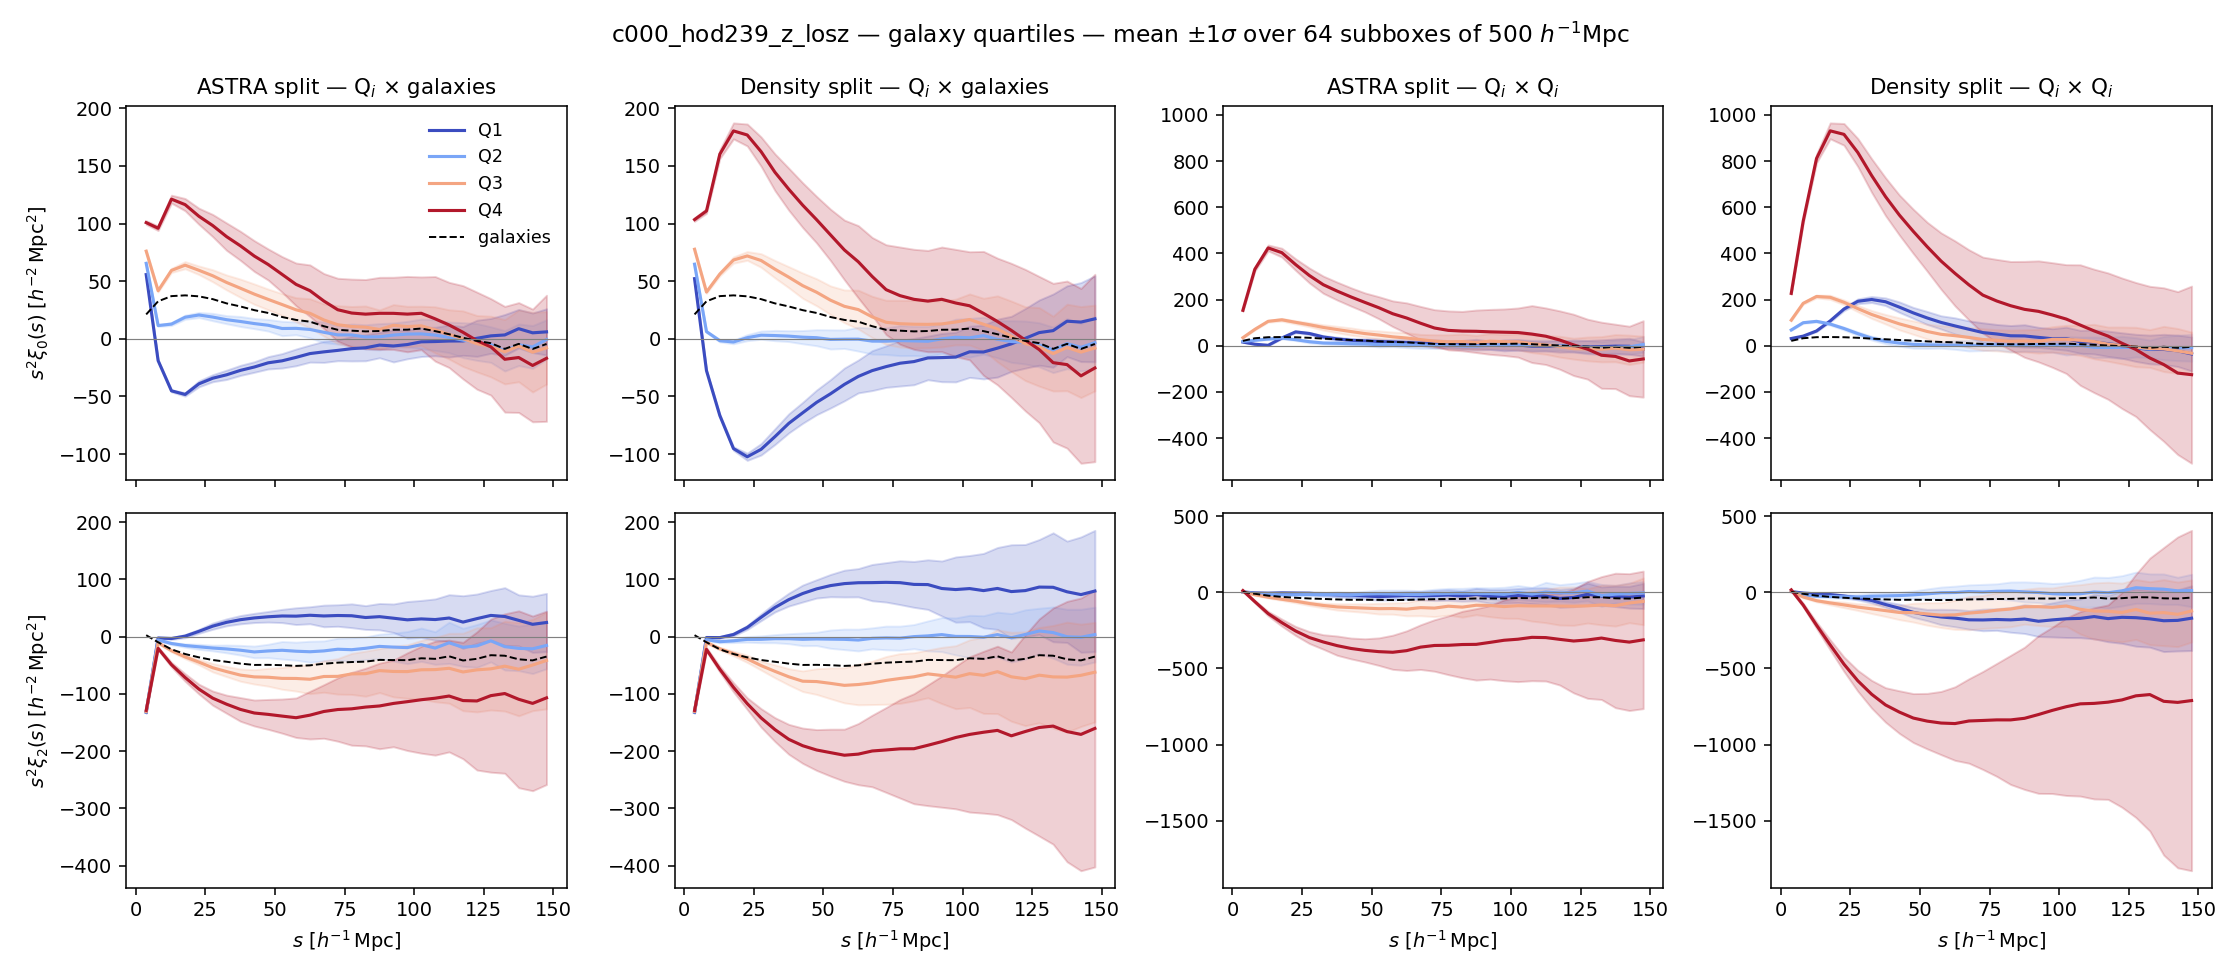
\includegraphics[width=\textwidth]{v2_multipoles_gal.png}
\caption{Same as Figure~\ref{fig:multipoles} for the galaxy quartiles.}
\label{fig:multipoles_gal}
\end{figure*}

\subsection{Real space and redshift space}

To isolate the effect of RSD, we also measured the fiducial catalogue (and the eight catalogues of the derivative pairs) in real space, the environments being then defined from the real-space positions (r-split) instead of the redshift-space ones (z-split), along the three lines of sight. Figure~\ref{fig:realz} compares the two. In redshift space, the monopoles at $20$--$60\Mpch$ are larger, by a factor 1.6 for the galaxy 2PCF and by 1.3--1.5 for the Q1 and Q4 cross-correlations of both methods. This is the Kaiser effect: galaxies fall coherently towards overdense regions and flow out of underdense ones, which in redshift space compresses structures along the line of sight and makes them look more contrasted, so that the real-space amplitudes are lower. The same flows create quadrupoles that vanish in real space: positive around underdense regions (outflows) and negative around overdense ones (infall). In absolute value the quadrupoles of density split are 1.6--1.7 times larger than those of ASTRA split, following their larger monopoles. Relative to the monopole, however, the ASTRA quadrupole is the larger one ($|\xi_2|/|\xi_0|\simeq0.8$ for ASTRA vs $0.6$ for density split for Q1, $1.0$ vs $0.8$ for Q4, at $20$--$60\Mpch$). A plausible explanation is that ASTRA defines environments from the nearest neighbours in redshift space, at a scale ($\sim13\Mpch$) at which the distortions are strong, so that its selection of environments is itself anisotropic, whereas the isotropic smoothing of density split partly averages the distortions out. The ASTRA environments are thus less contrasted but more sensitive, relative to their amplitude, to the velocity field. Real-space environments are not observable, so all the forecasts use z-split; the real-space measurements are kept as a diagnostic. (A first version of this work used real space as a ``truth'' to quantify ``systematic biases'' of redshift-space forecasts; since both measurements and emulator are in redshift space, this comparison does not describe a bias of the analysis, and the relevant systematic, the emulator error, is included in the covariance.)

\begin{figure*}[!tp]
\centering
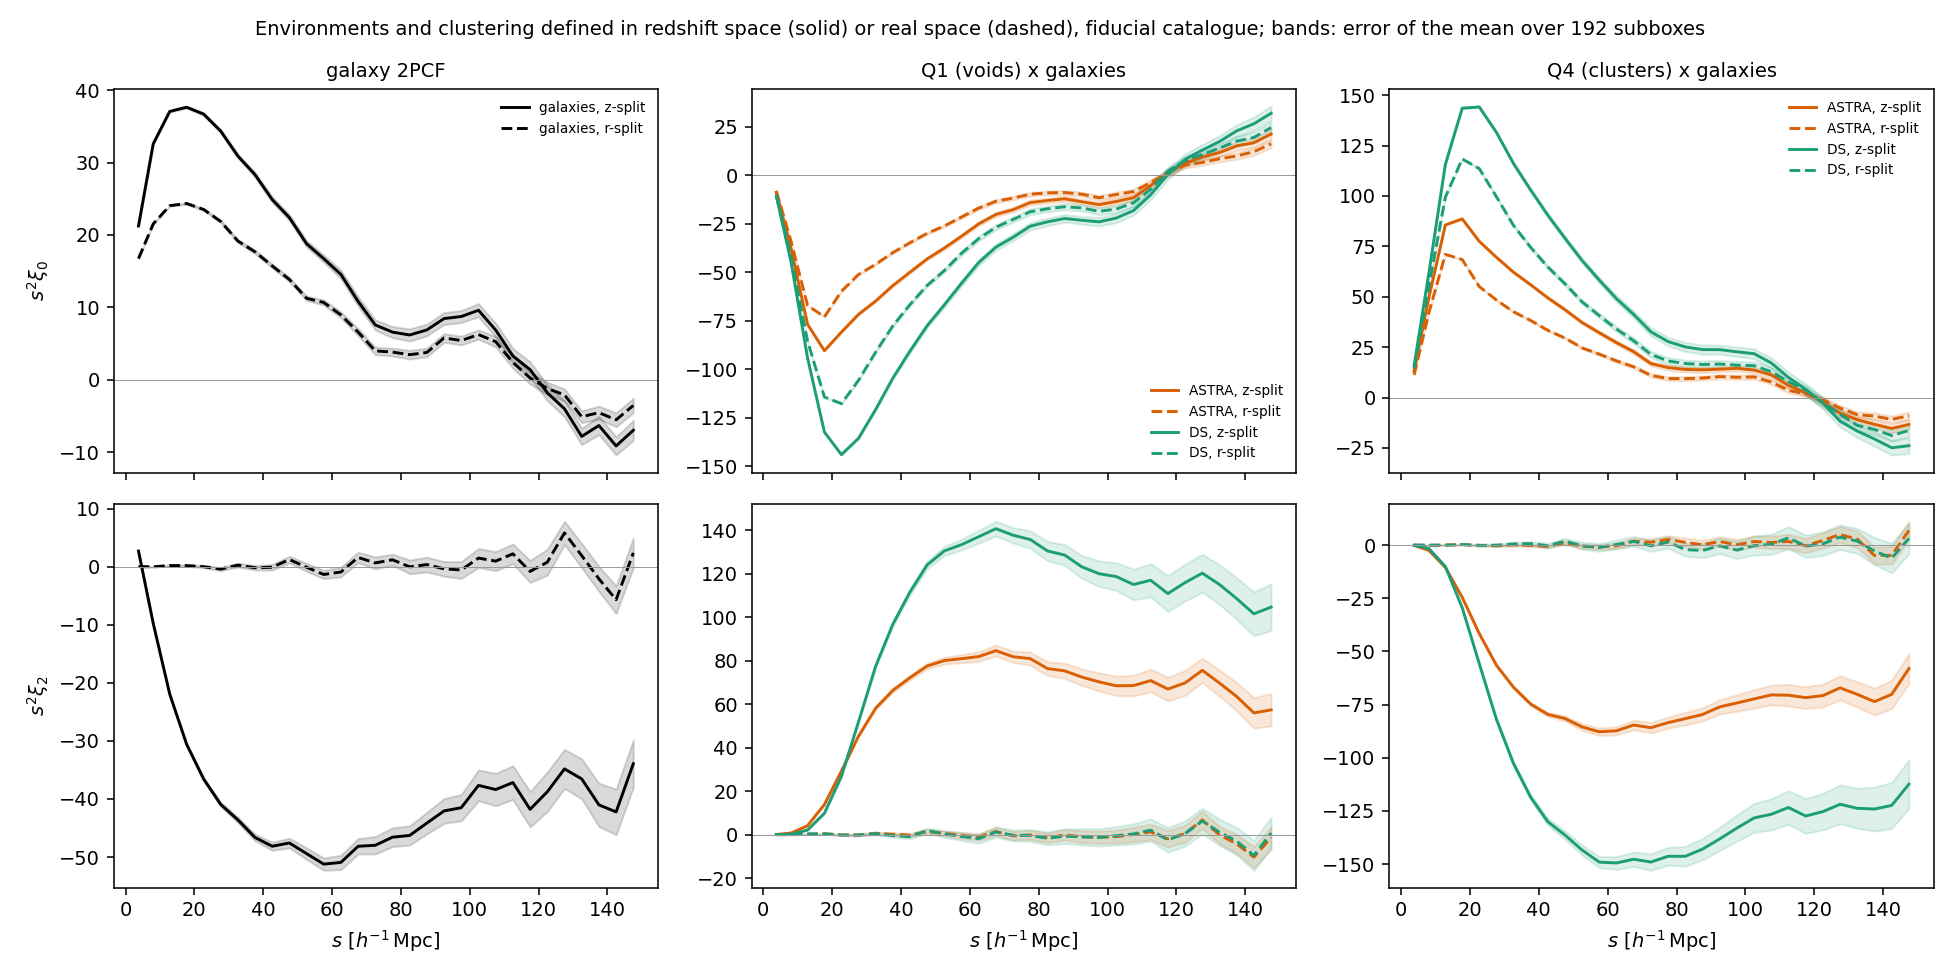
\includegraphics[width=\textwidth]{v2_real_vs_redshift.png}
\caption{Environments and clustering defined in redshift space (solid) or real space (dashed) for the fiducial catalogue: galaxy 2PCF (left), Q1 (centre) and Q4 (right) random-quartile cross-correlations of ASTRA split (orange) and density split (green). Top: monopole, bottom: quadrupole. Bands: error of the mean over $3\times64$ subvolumes.}
\label{fig:realz}
\end{figure*}


